\documentclass{article}

\usepackage[utf8]{inputenc}
\usepackage{parskip}
\usepackage{amssymb,amsfonts,amsmath,amscd}
\usepackage{bm}
\usepackage{hyperref}
\usepackage[pdftex]{graphicx}
\usepackage{url}
\usepackage[usenames,dvipsnames]{color}
\usepackage{enumitem}
\usepackage{mathtools}
\usepackage{float}

% for typesetting in-text numbers and units
\usepackage{siunitx}

% Table stuff.
\usepackage{booktabs}
\usepackage{makecell}
\usepackage{multirow}

% biblatex for bibliography
\usepackage[
backend=biber,
maxcitenames=1,
style=authoryear,
]{biblatex}

% \addbibresource{bibliography.bib}

\DeclareMathOperator*{\argmin}{argmin}

\title{Mobile Manipulation Calibration}
\author{Adam Heins}

\begin{document}

\maketitle

\section{Introduction}

The frames of interest are listed in Table~\ref{tab:frames}.

\begin{table}[h]
  \caption{Coordinate frames.}
  \centering
    \begin{tabular}{l c}
      \toprule
      Name & Subscript \\
      \midrule
      World        & $w$ \\
      Mobile base  & $b$ \\
      Base of arm  & $a$ \\
      End effector & $e$  \\
      Tool         & $t$ \\
      \bottomrule
    \end{tabular}
  \label{tab:frames}
\end{table}

The pose~$\bm{T}_{wt}$ of an arbitrary tool attached to the end effector can be
computed using the sequence of transforms
\begin{equation}\label{eq:kinematic_chain}
  \bm{T}_{wt} = \bm{T}_{wb}(\bm{q}_b)\bm{T}_{ba}\bm{T}_{ae}(\bm{q}_a)\bm{T}_{et},
\end{equation}
where~$\bm{T}_{wb}$ depends on the base
configuration~$\bm{q}_b=[x_b,y_b,\theta_b]^T$ and~$\bm{T}_{ae}$ depends on the
arm configuration~$\bm{q}_a$.

\section{Base Calibration}

We need to calibration the Vicon measured base poses~$\hat{\bm{q}}_b$ so that
the origin of~$\bm{T}_{wb}$ is correct. We have
\begin{equation}
  \bm{T}_{wb}(\bm{q}_b) = \begin{bmatrix}
    \bm{C}_z(\theta_b) & \bm{r}_b \\
    \bm{0}^T & 1
  \end{bmatrix},
\end{equation}
where~$\bm{C}_z(\theta)\in SO(3)$ is a rotation about the $z$-axis
and~$\bm{r}_b=[x_b,y_b,z_b]^T$ with~$z_b$ a constant. Our goal in this section
is to calibrate the origin~$(x_b,y_b)$ so that it is located at the point of
rotation of~$\theta_b$.

Starting at an arbitrary configuration~$\bm{q}_{b,0}$, we will move the base to
a sequence of desired yaw angles~$\theta^d_{b,i}$ and obtain the corresponding
measured configurations~$\hat{\bm{q}}_{b,i}$. We would like to find an
offset~$\Delta\bm{r}_b$ such that
\begin{equation}
  \bm{r}^d_{b,i} = \hat{\bm{r}}_{b,i} + \Delta\bm{r}_b
\end{equation}
is satisfied as closely as possible for each~$i$. We will do so by solving the
least squares problem
\begin{equation}\label{eq:contact_force_formulation}
  \argmin_{\Delta\bm{r}_b}\ \frac{1}{2}\sum_i\|\bm{r}_{b,0} - \hat{\bm{r}}_{b,i} - \Delta\bm{r}_b\|^2,
\end{equation}
where we've used the fact that~$\bm{r}^d_{b,i}=\bm{r}_{b,0}$.

\section{Arm--End Effector--Tool Calibration}

\begin{figure}[h]
  \centering
  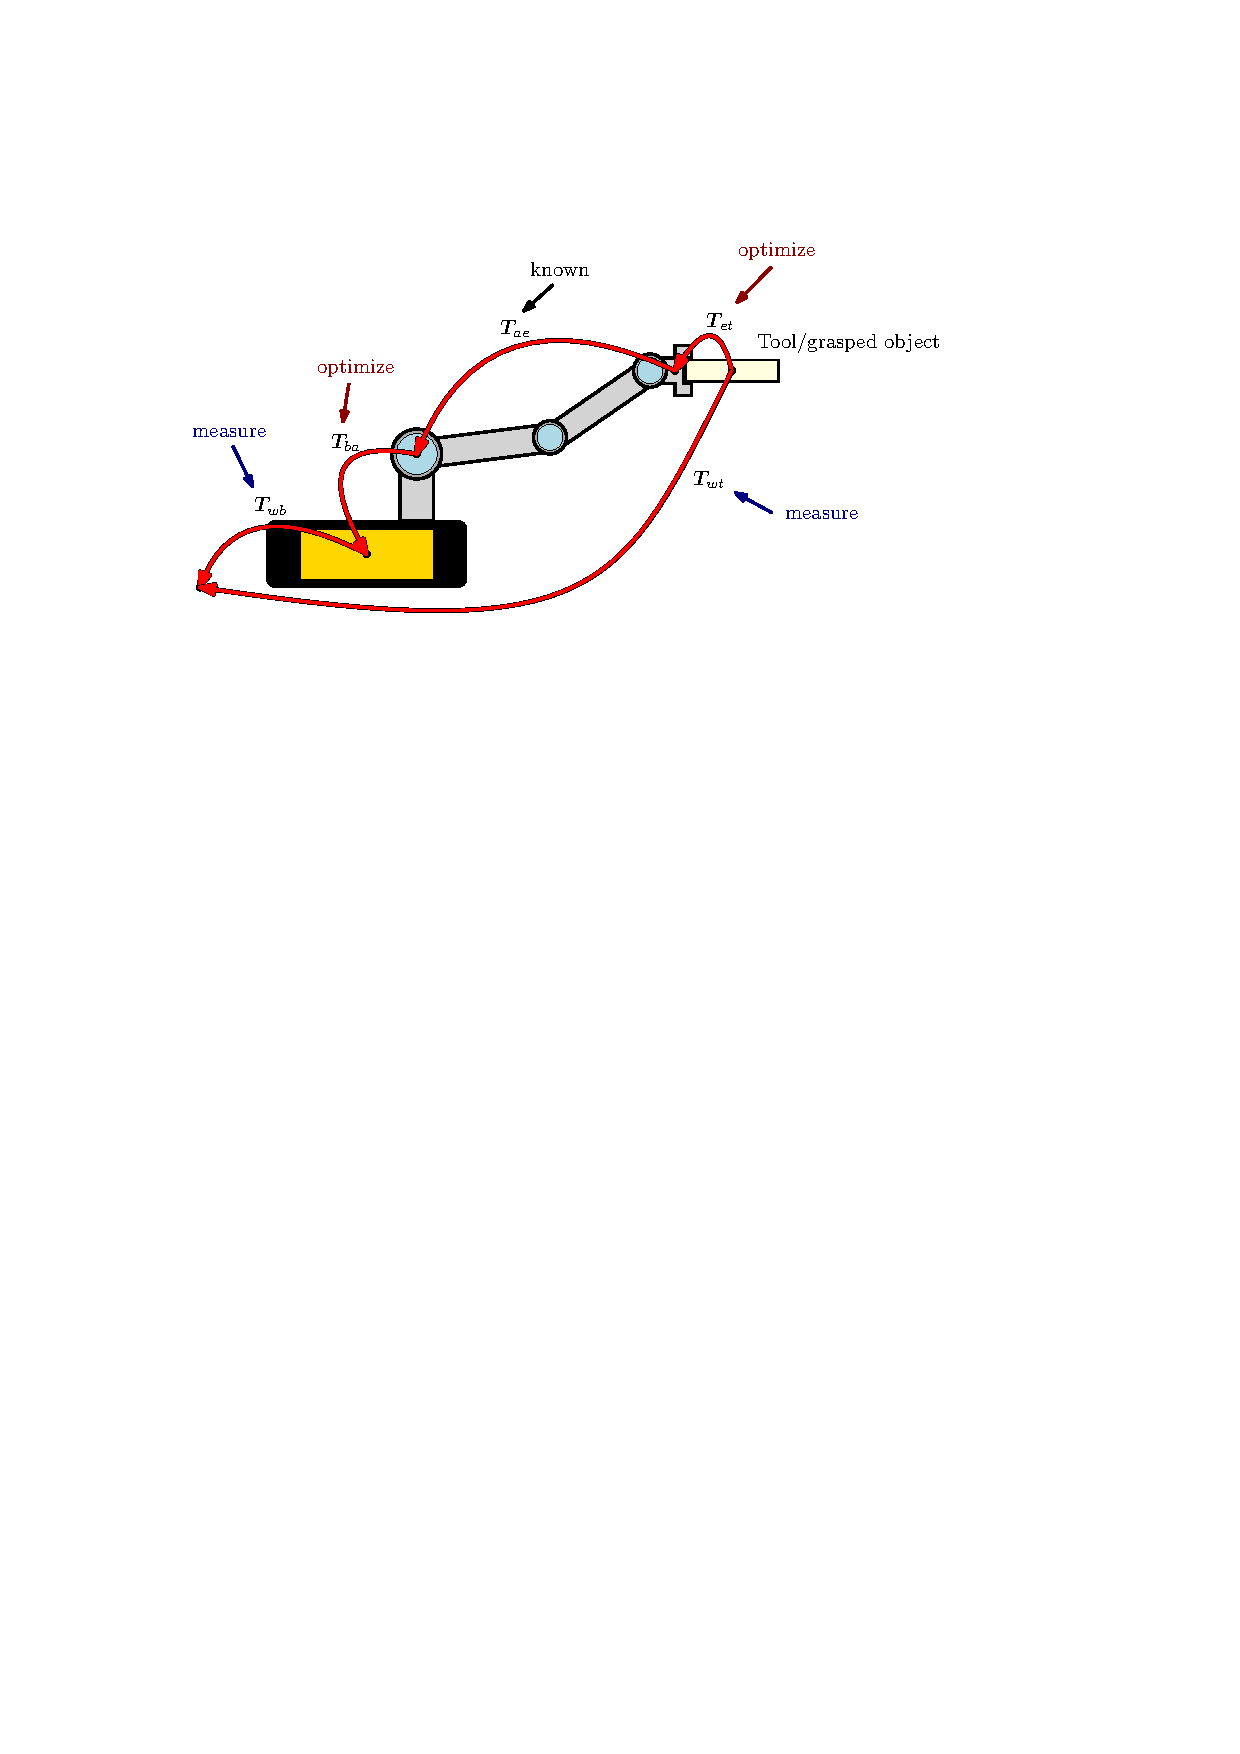
\includegraphics[width=1\textwidth]{figures/robot_calibration.pdf}
  \caption{Frames on the robot being calibrated.}
    \label{fig:calibration}
\end{figure}

Having calibrated the base pose~$\bm{T}_{wb}$, we now wish to calibrate
(static) the transforms between the base and arm~$\bm{T}_{ba}$ and the EE and
tool~$\bm{T}_{et}$. We will assume that factory calibration for the arm
transform~$\bm{T}_{ae}(\bm{q}_a)$ is good enough.

To do so, we will collect a sequence of
pairs~$(\bm{q}_{a,i},\hat{\bm{T}}_{wt,i})$ by moving the arm to the sequence of
configurations~$\bm{q}_{a,i}$. We will then solve the (nonlinear) least squares
problem\footnote{We may have nominal guesses for the transforms, in which case
we would actually optimize over (for example)~$\Delta\bm{T}_{ba}$,
where~$\bm{T}_{ba}=\Delta\bm{T}_{ba}\bar{\bm{T}}_{ba}$ with nominal
guess~$\bar{\bm{T}}_{ba}$.}
\begin{equation}
  \argmin_{\bm{T}_{ba},\bm{T}_{wt}}\ \frac{1}{2}\sum_i\|\boxminus(\bm{T}_{wt}(\bm{q}),\hat{\bm{T}}_{wt})\|^2.
\end{equation}
over the manifold~$SE(3)$, where~$\bm{T}_{wt}$ is computed using~\eqref{eq:kinematic_chain} and
\begin{equation}
  \boxminus(\bm{T}_1,\bm{T}_2) = \log(\bm{T}_1^{-1}\bm{T}_2)^\vee
\end{equation}
is the error between the poses.


\end{document}
